%!TEX root = ../main_wo_rep.tex
%
% 放射線の測定
%


\section{放射線の測定}


\subsection{原子核と放射線の種類}

原子の中心にはプラスの電荷を持った原子核が存在し、原子核は陽子と中性子で構成されています。
原子核を構成している陽子の数(プラスの電荷)のことを{\bf 原子番号}といい、
陽子と中性子の数を合わせたものを{\bf 質量数}といいます。

原子番号が同じで化学的な性質が同じであっても、質量数が異なる原子が存在し、お互いを{\bf 同位体(アイソトープ)}と呼びます。これら同位体を区別するために、元素名に続けて質量数を示し「炭素12」のように表すか、元素記号の左肩に質量数を書いて${}^{12}{\rm C}$と表します。(原子番号は元素の種類と対応しており、元素記号から一意に定まります。)

同位体の原子核の中には不安定なものがあり、放射線やエネルギーを放出します({\bf 放射性崩壊})。
放射線を出す性質(放射能)を持った同位体のことを放射性同位体と呼びます。
放射性同位元素から放出される放射線はその種類により、α線(ヘリウム原子核)、β線(電子)、X線およびγ線(電磁波)などに分類されます。
また、核分裂反応によって生じる中性子線も放射線の一種です。
放射線は一般に高いエネルギーを持つため、大量に浴びると放射線障害と呼ばれる影響が身体に現れることがあります。

\subsection{放射能および放射線の単位}

放射能を持つ1つの原子核がいつ放射性崩壊を起こして放射線を出すのかは量子力学的現象であるため確率的にしか予測できませんが、
その原子核が多数集まることで統計的な量を定義することができます。
特に、同じ種類の多くの放射性同位元素を集めた時、その原子核が放射性崩壊を起こして他の元素に変化してその数が半分になる時間を半減期
という量で表します。
半減期が短いとは、放射性同位体が早い時間で崩壊していくことを意味していて、
その原子核が非常に不安定であることを表します。反対に、
半減期が長い放射性同位体はより安定であると言えます。

放射性同位元素の原子核が1秒間に崩壊する原子核の個数をベクレル[Bq]という単位で表します。
当然、原子核の数が多ければ多いほど1秒あたりに崩壊する原子核の個数(ベクレル)は大きくなるので、
同じ量で比較する場合には、1Lあたり[Bq/L]や1kgあたり[Bq/kg]といった単位を用います。

放射線はその種類やエネルギーによって物質への吸収のされ方(エネルギーの与え方)が異なっています。
放射線が
物質1kgにつき1Jの仕事に相当するエネルギーを与えた(吸収された)とき、
その量を測る単位(吸収線量)として、1グレイ[Gy]を定義します。

さらに、同じ吸収線量であっても放射線の種類によっては人体へ対する影響が同じとは限りません。
そのため、放射線障害からの防護という観点からは、放射線源の場所、受けた放射線の種類、対象組織などの違いによって
修正係数を乗じて補正を行った線量当量(シーベルト[Sv])という単位を用います。
(完全に科学的な理由で定義された単位ではなく、法令などで規定された単位です。)
ただし、X線、γ線、β線など測定で主要な放射線の修正係数は1であるので、今回の測定の際には線量当量(Sv)と吸収線量(Gy)
は同じものと思って差し支えありません。

\subsection{放射線の測定方法}

放射線は{\bf 電離作用}と呼ばれる通過している物質中の電子を弾き飛ばして電離させる作用があります。
放射線を検出するにはこの電離作用を用います。

ガイガー=ミュラー検出器はヘリウム、ネオン、またはアルゴンといった不活性ガスを封入した管の中に電極を設置したものです。
電極に数百ボルトの高電圧をかけておくと、通常は電極間に電流は流れませんが、管の中を放射線が通過すると
中の不活性ガスが電離し、電子なだれという現象によって電流が流れます。
単位時間ごとに電流が流れた回数を数えると、管を通過した放射線の個数を知ることができます。
この単位時間あたりの個数から、グレイやシーベルトといった値を測定します。

ガイガー=ミュラー検出器では通過した放射線の個数(線量)しかわからず、放射線ごとのエネルギーを測定することはできません。
そのため、どのような原子核が崩壊して、どのようなエネルギーの放射線が放出されたのか特定するためにはシンチレータと呼ばれる
物質を使った検出器を用います。
シンチレータとしてヨウ化セシウム(CsI)やヨウ化ナトリウム(NaI)などの無機結晶を用いることが多いですが、プラスチックや液体・気体状のものもあります。
このような結晶中を放射線が通過すると、そのエネルギーを吸収し、蛍光と呼ばれる光を発します。
放射線1つでの発光は非常に弱いものですが、そのわずかな光を光電子増倍管や半導体を用いたセンサーを使って検出します。
入射した放射線のエネルギーと蛍光の強度(明るさ)はほぼ比例関係にありますので、発光の明るさを測定すれば放射線のエネルギーを
知ることができます。

シンチレータからの光を検出し、測定するには光電子増倍管がかつては主に使われていましたが、
現在は半導体技術の進歩によりMPPC(Multi-Pixel Photon Counter)などの半導体を用いた小型のセンサーが用いられるようになりました。
今回の実験ではタリウム活性化ヨウ化セシウムをシンチレータ、MPPCを光センサーとして用いた検出器で測定を行います。

\subsection{自然界における放射線}

放射線は原子力発電所や核兵器などで人工的に作られたものだけと思いがちですが、我々は日常的に自然界にもともと存在する放射線を受けています。
自然界に存在する放射線としては、ラドン222やカリウム40などの天然放射性核種や宇宙から飛来する宇宙線などがあります。
日本国内ではこれらの自然放射線から年間2.1mSv程度被ばくしていると言われています。

ラドン222は岩石中に含まれるウラン238やラジウム226から放射性崩壊によって生成した大気中に存在する希ガスで、
さらにラドン222から放射性崩壊して生成される鉛214やビスマス214も放射性同位体となります。
一方、カリウム40は放射線を出さない安定なカリウムに対して、自然界に約0.01\%の割合で存在する放射性同位体です。
カリウムは人体に必要な元素のため、私たちは体内からもカリウム40由来の放射線を常に受けています。

宇宙から飛来する放射線の由来は様々ですが、その発生原因や性質を調べることで遠い宇宙での出来事や素粒子の成り立ちが分かるため、
最先端の物理学の研究にとても役立っています。

\newpage

\jikken

\begin{itemsquarebox}[c]{\bf 実験用具}
放射線検出モジュール、パソコン、放射線源試料、鉛シート
\end{itemsquarebox}

\bigskip

\subjikken{放射線源試料のエネルギースペクトルの測定}

\begin{enumerate}

\item 放射線検出モジュールとパソコンをUSBケーブルで接続します。

\item 放射線検出モジュールのシンチレータ部分に放射線源試料を近づけ、鉛シートで包みます。

\item 放射線検出モジュール用のアプリケーションソフトを立ち上げ、測定を開始します。測定時間は1時間に設定します。

\item 測定後、出力されたデータ(CSVファイル)をエクセルに読み込み、横軸をエネルギー(30keV$\sim$2000keV)、縦軸をカウント数(対数軸)
としたグラフを作成します。

\item グラフから放射線のエネルギースペクトルを読み取ります。放射線源試料にはトリウム232(${}^{232}{\rm Th}$)
という放射性同位体が含まれています。トリウム232が崩壊して生成する元素、およびそこから発生するγ線のエネルギーを参考にして、
測定したエネルギースペクトルの放射線(γ線)がどの放射性同位体から生じたものか、同定してみましょう。



\end{enumerate}

\paragraph{注意}
放射線源として用いる試料は一般用途として店頭販売されているものなので、危険性はありませんが、
取り扱い上の注意は必ず守るようにしましょう。

\newpage

\paragraph{参考1}
トリウム232の崩壊系列図
\begin{center}
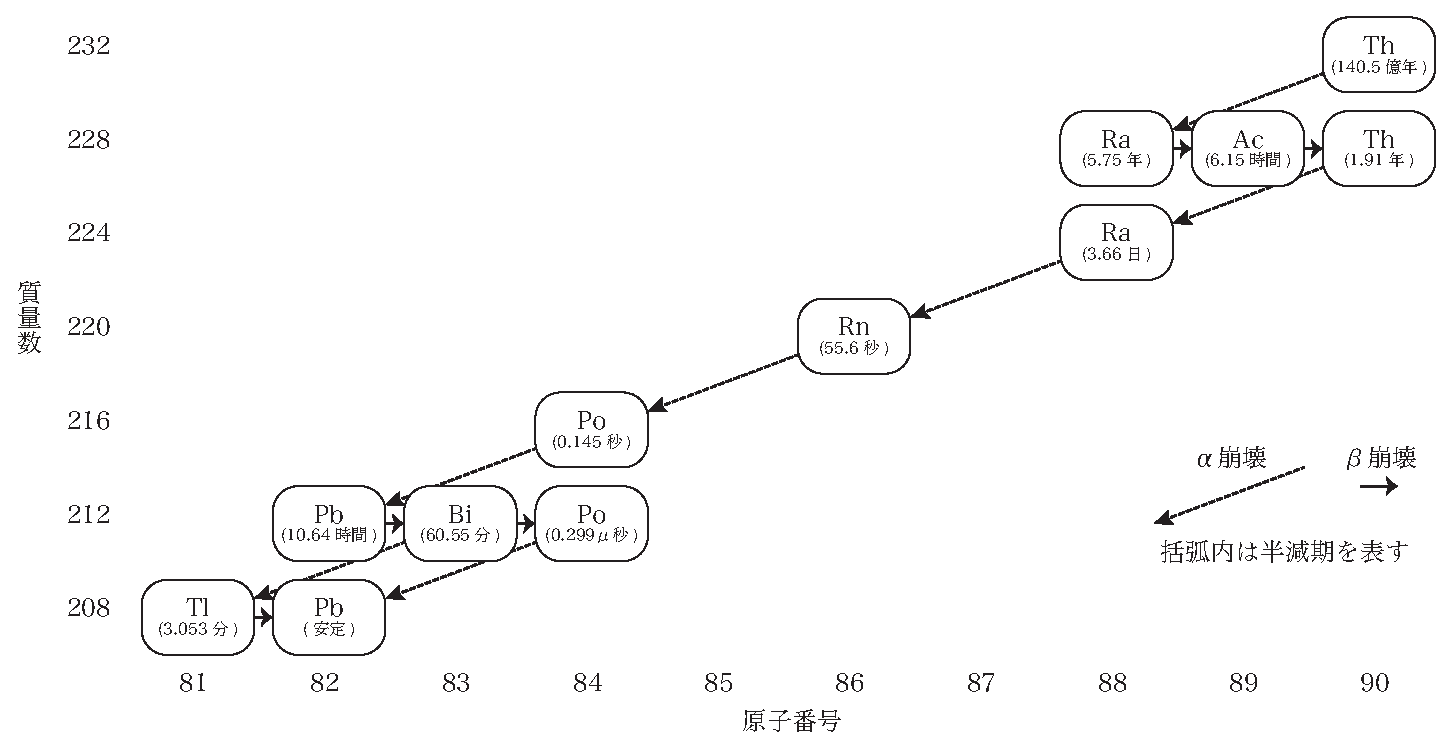
\includegraphics[width=155mm]{14_Radiation/Thorium.eps}
\end{center}


\paragraph{参考2}
トリウム232の崩壊生成物から出る主なγ線のエネルギー\\
\begin{tabular}[t]{|c|r|r|}
\hline
放射性同位体 & γ線のエネルギー& 強度\\
& [keV] & \\
\hline\hline
${}^{228}$Ac & 99.509 & 1.26\\
& 129.065 & 2.42\\
& 209.253 & 3.89\\
& 270.245 & 3.46\\
& 328.000 & 2.95\\
& 338.320 & 11.27\\
& 409.462 & 1.92\\
& 463.004 & 4.40\\
& 755.315 & 1.00\\
& 772.291 & 1.49\\
& 794.947 & 4.25\\
& 835.710 & 1.61\\
& 911.204 & 25.80\\
& 964.766 & 4.99\\
& 968.971 & 15.80\\
& 1588.200 & 3.22\\
& 1630.627 & 1.51\\
\hline
\end{tabular}
\begin{tabular}[t]{|c|r|r|}
\hline
放射性同位体 & γ線のエネルギー& 強度\\
& [keV] & \\
\hline\hline
${}^{212}$Pb & 238.632 & 43.3\\
& 300.087 & 3.28 \\
\hline
${}^{212}$Bi & 39.857 & 1.06\\
& 727.330 & 6.58\\
& 785.370 & 1.10\\
& 1620.500 & 1.49\\
\hline
${}^{208}$Tl & 277.358 & 6.31\\
& 510.770 & 22.60\\
& 583.191 & 84.50\\
& 763.13 & 1.81\\
& 860.564 & 12.42\\
& 2614.533 & 99.16\\
\hline
\end{tabular}
